\documentclass[10pt,a4paper]{article}
\usepackage[margin=1.8cm]{geometry}
\usepackage{fontspec}
\setmainfont{Helvetica Neue}[Scale=0.95]
\usepackage{graphicx}
\usepackage{booktabs}
\usepackage{xcolor}
\usepackage{hyperref}
\usepackage{titlesec}
\usepackage{enumitem}
\usepackage{caption}
\hypersetup{colorlinks=true,urlcolor=blue!60!black,linkcolor=black}
\titleformat{\section}{\normalsize\bfseries}{}{0pt}{}
\titlespacing{\section}{0pt}{9pt}{3pt}
\setlength{\parskip}{4pt}
\setlength{\parindent}{0pt}
\captionsetup{font=small,labelfont=bf,skip=3pt}
\pagestyle{empty}

\begin{document}

{\large\bfseries LFP2Vec across labs: a reproduction, a preprocessing fix, and a calibration check}

\vspace{2pt}
{\small Keshav Rajput, September 2026. Code, data manifests, exact splits and every number below:
\url{https://github.com/happyc0der/lfp2vec-audit}. Corrected 21 September 2026; see the README.}

\section{Question}
LFP2Vec (He et al., NeurIPS 2025) fine-tunes an audio model on raw local field potential to
predict which brain region an electrode sits in, and reports zero-shot transfer between labs. Its
Broader Impact section states that clinical use ``should include calibrated uncertainty
estimates''. This note reproduces the fine-tuning stage on the two public datasets the paper uses,
asks why cross-lab transfer failed in the reproduction, fixes it, and measures calibration under
lab shift, which the paper does not report.

\section{Setup}
\textbf{Data.} Seven IBL insertions from five labs and ten Allen Visual Coding probes, chunked as
the released code does: three seconds, one hundred chunks per channel. 132\,600 IBL and 50\,200
Allen chunks. Two Allen probe files that contain only zeros were excluded; IBL contains no CA2
channels, so results use four classes.
\textbf{Method.} \texttt{facebook/wav2vec2-base} fine-tuned with the paper's hyper-parameters. The
self-supervised continuation is not run; in the released code it runs per dataset and never sees
two labs. No pretrained weights are available, so published numbers are read from figures
($\pm$0.01).
\textbf{Evaluation.} Leave-one-session-out within lab; across labs, train on one and score every
probe of the other. Balanced accuracy with chance computed from the classes each test set
contains, and raw accuracy over the majority-class rate where the paper uses that. Permuted-label
controls on every fold sit at chance.

\section{Results}
\textbf{1. Within a lab it reproduces.} 0.72 balanced accuracy on held-out IBL sessions against
the paper's 0.68; with the paper's post-processing, 0.76. Fine-tuning adds 0.007 over the
untrained audio checkpoint with a linear head, and replacing inputs with surrogates that keep the
power spectrum and destroy the waveform costs 0.008: on this task the model reads spectral power.
It beats six-band power by 0.24.

\textbf{2. Across labs the full-band model collapses, confidently.} It predicts one class for 94\%
of the other lab's chunks at 0.98 confidence, landing below the majority rate in both directions.
A linear probe recovers the source lab from its embeddings at AUC 0.997 on unseen probes. The
source is measurable: the datasets' spectra agree below 100\,Hz and diverge up to 768-fold above
300\,Hz, because one pipeline band-passes and the other does not.

\textbf{3. Matching the filters restores transfer.} Low-passing every input at 100\,Hz, a corner
fixed before any cross-lab result existed, with no labels from the target lab:

\begin{table}[h]
\centering\small
\begin{tabular}{lrr}
\toprule
raw accuracy minus majority-class rate & IBL $\to$ Allen & Allen $\to$ IBL \\
\midrule
LFP2Vec as published \textit{(Figure 2e)} & +0.11 & +0.12 \\
fine-tuned, full band & $-$0.03 & $-$0.06 \\
\textbf{fine-tuned, filters matched, + paper's post-processing} & \textbf{+0.15} & \textbf{+0.12} \\
band power + paper's post-processing & +0.17 & +0.03 \\
electrode position & $-$0.24 & 0.00 \\
\bottomrule
\end{tabular}
\end{table}

Balanced accuracy goes from 0.24 and 0.26 to 0.46 and 0.37 (0.56 and 0.36 post-processed), the
best of any method tested; lab identity falls to 0.83 and 0.74. Ruled out along the way: the
paper's post-processing alone (0.004 on a collapsed model), per-probe embedding centering (removes
the lab signature, leaves transfer at chance), and whitening each probe's whole spectrum (worse
than the low-pass in both directions).

\begin{figure}[h]
\centering
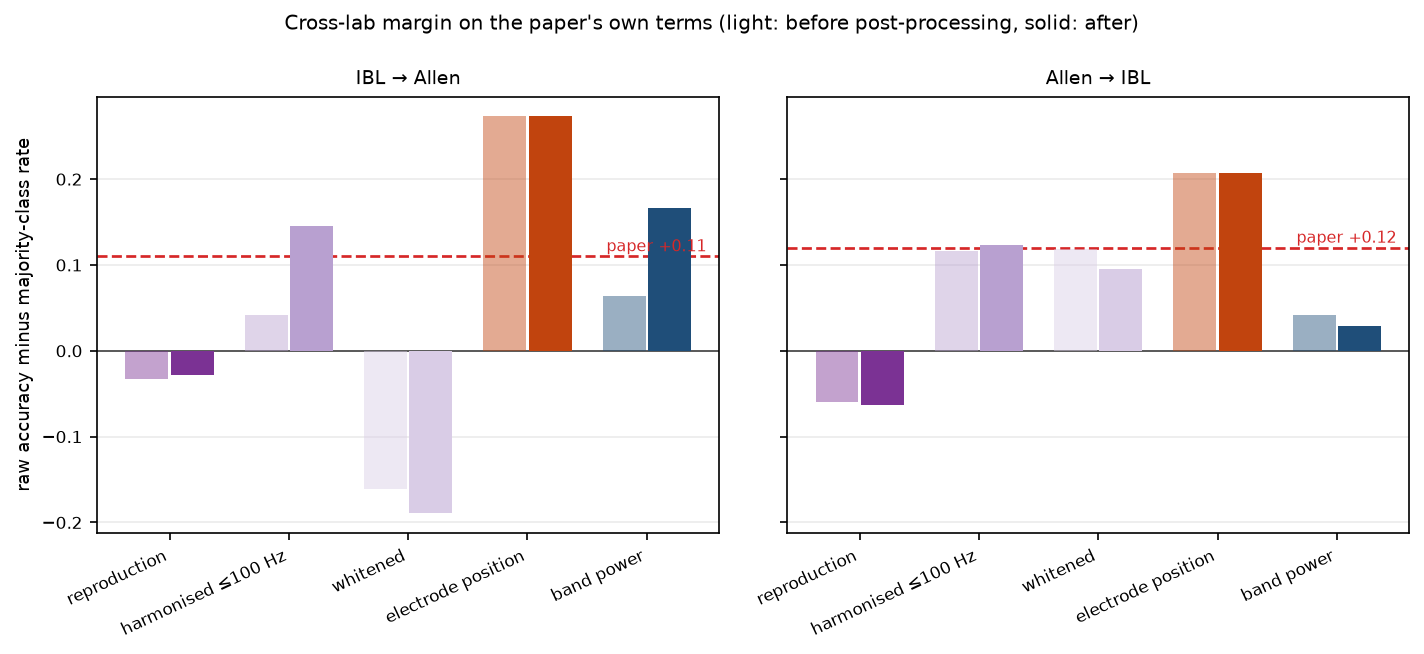
\includegraphics[width=0.86\textwidth]{../docs/figures/fixes.png}
\caption{Cross-lab margin on the paper's own metric. Light bars before the paper's
post-processing, solid after; dashed line is the published margin.}
\end{figure}

\textbf{4. Calibration does not survive the shift.} Expected calibration error is 0.10 in lab and
0.56 across labs. A temperature fitted in lab cuts the former to 0.03 and moves the latter to
0.51; the target lab needed a temperature four to seven times larger, which requires the labels
zero-shot transfer avoids. Matching the filters halves the cross-lab error (0.35) and makes
distance from the training distribution a working abstention score in both directions.

\textbf{5. Signal and position are complementary.} Depth along the shank alone reaches 0.77 on
IBL, where insertions are stereotyped, 0.49 on Allen, and chance across labs. Fused with the
signal as a product of experts it is at or above both parts. When insertion depth is uncertain,
position falls (0.75 $\to$ 0.63 at $\pm$400\,\textmu m on IBL) while the signal stays at 0.68: the
signal is the better single source beyond about $\pm$280\,\textmu m.

\section{What this says, and one next experiment}
The reduced method does what the paper reports within a lab. Its cross-lab failure here was
preprocessing the two datasets do not share, not the representation, and one line of filtering
recovers the published margin. Confidence is the part that does not transfer, and the measurement
the paper calls for is the one that shows it.
\textbf{Next.} Run the paper's full pipeline, self-supervision included, on inputs harmonised
first, and report calibration error beside accuracy. If lab identity stays near 0.8 the residual
is physiology; if it falls toward 0.5, acquisition was the whole story.

\section{Limitations}
Two of the paper's four datasets are private and untested. Labels are histological estimates taken
as given. Fine-tunes have three within-lab sessions and one seed per configuration so far; more
are training. Published numbers are read from bitmaps. An earlier version of this note reported a
position baseline that leaked test labels; it is corrected here. Much of the code was generated
with Claude; every experiment, split and number was independently checked.

\end{document}
